% ============================================================
% 中文版：面向工业智能体的语义感知时间敏感网络调度机制研究
% 基于英文版 main.tex 的完整中文翻译
% ============================================================
\documentclass[UTF8]{ctexart}
\usepackage{amsmath,amssymb,amsfonts}
\usepackage{algorithmic}
\usepackage{graphicx}
\usepackage{textcomp}
\usepackage{xcolor}
\usepackage{booktabs}
\usepackage{array}
\usepackage{multirow}
\usepackage{hyperref}
\usepackage[top=2.5cm,bottom=2.5cm,left=2.5cm,right=2.5cm]{geometry}

\title{语义感知时间敏感网络调度：约束安全强化学习方法}
\author{
    胡海超\\
    \small Comm-AI.tech 独立研究者\\
    \small 中国成都\\
    \small haichao.hu@comm-ai.tech
}
\date{}

\begin{document}

\maketitle

% ============================================================
\begin{abstract}
% ============================================================

现有时间敏感网络（TSN）调度几乎完全以网络层指标（吞吐、抖动、端到端时延）为优化目标，忽略了工业智能体任务的语义——同一传感器流在"巡检"和"急停"两种任务上下文中，延迟容忍度相差三个数量级。这种语义鸿沟导致网络资源分配与智能体真实需求错配。

本文提出首个语义感知 TSN 调度框架，包含三个核心组件。其一，任务意图本体，将六类工业任务（巡检、协同、急停、周期控制、遥测、重配置）经四级关键性（L0--L3）映射为流语义描述——优先权权重、紧迫性函数、可延迟边界——进而转化为门控列表（GCL）和基于信用整形器（CBS）参数。其二，约束安全强化学习（CSRL）调度器，将调度问题建模为 Lagrangian 约束马尔可夫决策过程，以语义加权任务完成率为奖励，以网络演算（NC）最坏情况延迟（WCD）上界为可学习约束。其三，NC 安全盾在每次调度动作执行前进行确定性可调度性验证，提供与策略无关的分关键性级别容忍策略。

在 3 交换机线形拓扑、10 ms 超周期（与流周期同尺度）的仿真环境中，经三种实验模式验证：静态基准（5/8/12 流）、动态流到达（5 基站 + 3 到达）、组件消融。CSRL 调度器在 5 流和 8 流下达 100\% 任务完成率，12 流下达 97.5\%（多种子 92.8\% $\pm$ 3.6\%），接近静态贪心 GCL 基线（静态场景均 100\%），同时无需离线重配置即可支持动态流到达。Lagrangian 乘子 $\lambda$——它将网络演算约束耦合进学习目标——随流量密度单调上升（5 流 0.12 至 12 流 0.67），证明形式化约束压力真实传导至学习策略。消融研究确认 Lagrangian 机制处于激活状态（完整 CSRL $\lambda=0.29$ 对比约束禁用 $\lambda\equiv0$），且语义加权更强地激活约束项（无语义 $\lambda=0.10$）。此外，在窗口时隙稀缺的极限场景（10 条同周期流单端口竞争）中，CSRL 与纯 DRL 均达 100\% 完成率，而静态贪心互斥分配仅 41.7\%——协调多同周期流正是贪心启发式的组合短板。这些结果表明语义感知、可形式化验证的 RL 调度架构在性能上与经典调度器可比，同时保留在线适应能力。

\textbf{关键词：}时间敏感网络；语义感知调度；约束强化学习；网络演算；意图驱动网络

\end{abstract}

% ============================================================
\section{引言}
% ============================================================

工业自动化正经历从确定性周期控制——PLC 以固定间隔轮询传感器并指令执行器——向 AI 智能体驱动的分布式协同的范式转变。自主移动机器人、协作机械臂和数字孪生系统基于语义上下文协商任务，而非依赖预先配置的调度表。时间敏感网络（TSN），经由 IEEE 802.1 一系列子标准标准化，为这一转变提供了确定性通信基础：时间感知整形（TAS, 802.1Qbv）通过门控列表（GCL）隔离关键流量；帧抢占（802.1Qbu/802.3br）将保护带压缩至 1 Gbps 链路上约 0.6 $\mu$s；广义精确时间协议（gPTP, 802.1AS-2025）在七跳内提供亚微秒级同步精度。

然而现有 TSN 调度方法，包括最前沿的强化学习方案，共享一个共同的盲点：它们仅优化网络层关键性能指标——端到端延迟、抖动、吞吐——而不建模数据对消费它的应用层意味着什么。这在工业智能体场景中产生了三种结构性的错配：

\begin{enumerate}
\item \textbf{语义错配。} 网络优先级（PCP 0--7）与任务关键性并不一一对应。一条 PCP~5 的 LiDAR 扫描流在仓库巡检时承载常规环境数据，但在检测到障碍物时成为安全关键信号——然而 TSN 调度器在帧头中看不到任何区别。
\item \textbf{静态-动态错配。} GCL 在已知、固定流集的假设下离线计算。而工业智能体任务会随环境事件动态到达、终止和改变关键性。
\item \textbf{可证性错配。} 学习型调度策略——无论来自深度 RL 还是大语言模型（LLM）——不能提供 WCD 的形式化保证。在受 ISO 26262 ASIL-D 或 IEC 61508 SIL 管辖的安全关键领域，概率性保证是不充分的。
\end{enumerate}

第三个错配已有令人警醒的量化证据。Debnath 等人开发了 TSNBench~\cite{debnath2026tsnbench}，首个在 TSN 领域评估 LLM 能力的基准，在 16 个模型上测试了 939 道多选题和 100 道开放式 WCD 计算题。多选题正确率为 67\%--95\%，但 WCD 计算方面全面崩溃：在基于信用整形器（CBS）分析中，最优模型仅达 36.2\% 的平均绝对百分比误差（MAPE），大多数模型超过 80\%；在循环排队和转发（CQF）中，最优 MAPE 为 41.8\%。这些误差并非学术数字——在真实 WCD 为 100 $\mu$s 的运动控制回路中，36\% 的低估意味着系统错误地认证了一个将超出截止时间 36 $\mu$s 的调度配置。TSNBench 的核心发现是：对 TSN 标准的概念性熟悉（由多选题衡量）并不能转化为 WCD 分析所需的精确多步数学推导。LLM 不能单独承担安全关键的 TSN 调度决策。

这一发现同样适用于深度 RL 调度器。Islam 和 Muslim 的 GCN-TD3~\cite{islam2024gcntd3}——当前最强的纯 DRL TSN 调度器之一——通过图卷积网络状态嵌入和 TD3 连续动作优化维持 90\% 的动态流接纳率。但其安全机制是基于 ILP 的系统级重启（当 GCL 条目饱和时触发）——一种粗粒度的紧急制动，而非逐决策的验证门。现有 RL 调度器均不提供形式化 WCD 保证。

我们通过一个统一框架同时处理这三种错配。本文贡献如下：

\begin{enumerate}
\item \textbf{首个语义感知 TSN 调度范式。} 定义三层任务意图本体（意图 $\rightarrow$ 流语义 $\rightarrow$ TSN 参数），将工业智能体任务到 GCL 和 CBS 配置的映射形式化，弥合语义-网络表征的空隙。
\item \textbf{混合 AI-符号安全调度架构。} 组合 PPO 基约束安全 RL 调度器与网络演算安全盾——在每次动作执行前以确定性可调度性约束（窗口装帧、端口内窗口互斥、对齐截止时间可满足）验证每个动作，将学习策略的适应性与符号规则的确定性耦合。
\item \textbf{语义-网络双目标优化。} CSRL 奖励函数同时优化语义加权任务完成率和网络层延迟，表明语义加权奖励在保持与均匀奖励性能持平的同时，将 NC 约束耦合进学习目标。
\end{enumerate}

在 3 交换机线形拓扑实验中，CSRL 在 5 流和 8 流下达 100\% 任务完成率，12 流下达 97.5\%，接近静态贪心 GCL 基线（静态场景均 100\%），同时无需离线重配置即可支持动态流到达。形式化层的贡献可测量地体现在 Lagrangian 动力学中：$\lambda$ 从 5 流的 0.12 升至 12 流的 0.67，消融显示 NC 约束项主动塑造策略（完整 CSRL $\lambda=0.29$ 对比约束禁用 $\lambda\equiv0$）——形式化验证不仅是加在学习策略上的安全证书，而是优化目标的集成组件。在窗口时隙稀缺的极限场景下，RL 方法（CSRL/纯 DRL）达 100\% 完成率而静态贪心仅 41.7\%，展现了学习式协调对贪心碎片化的优势。

% ============================================================
\section{相关工作}
% ============================================================

\subsection{经典 TSN 调度}

TAS 调度的形式化基础由 Craciunas 等人~\cite{craciunas2016smt} 建立，他们将 IEEE 802.1Qbv GCL 合成为一个约束系统，涵盖四个域：帧约束（链路上窗口对齐）、链路约束（出口端口互斥）、流传输约束（跨跳空间-因果递进）、隔离约束（防止低优先级干扰的保护带）。其 SMT/ILP 双求解器方法对最多约 200 帧可实现最优调度，超过此规模则因底层无等待作业车间调度问题的 NP 难性而使精确方法失效。这一约束系统至今仍是所有后续 TSN 调度器——启发式、元启发式和学习型——的数学基准。Xue 等人~\cite{xue2024survey} 系统综述了 17 种 TSN 实时调度方法，确认了精确度-可扩展性折衷的根本性：精确方法（SMT, ILP, OMT）保证最优但扩展性差；启发式方法（贪心、列表调度）扩展性好但缺乏最优性界；学习型方法占据中间地带，但安全裕度未被量化。

\subsection{AI 和强化学习用于 TSN}

深度 RL 在 TSN 调度中的应用自 2022 年以来加速。Guo 等人~\cite{guo2024dirt} 提出 DiRTS，首个面向 802.1Qbv 的分布式多智能体 DRL 框架，相比 SOTA 调度成功率提升 20.31\%，大规模网络传输成本降低 410$\times$。Sun 等人~\cite{sun2024gatppo} 结合图注意力网络（GAT）与 PPO 用于车载 TSN，链路故障场景下 3.8 秒生成调度方案。Islam 和 Muslim~\cite{islam2024gcntd3} 将图卷积网络（GCN）与 TD3 集成用于连续动作动态调度，在小拓扑上实现约 90\% 动态流接纳率和 2 $\mu$s 抖动。Kim 等人~\cite{kim2024drl} 将 DRL 扩展到无线 TSN（IEEE 802.11），满足 99.9\% 延迟要求。Debnath 等人~\cite{debnath2025tta} 将 PPO 应用于流量类型分配问题，将其建模为 NP 难搜索空间上的学习任务。

这些方法共享两个局限。其一，优化目标纯属网络中心：流接纳率、平均延迟、抖动，无一将任务层紧迫性或语义优先级纳入奖励结构。其二，安全机制——即便存在——也是粗粒度的：Islam 和 Muslim 的 ILP 回退在 GCL 条目饱和时触发全系统重启；其他方法完全不提供形式化延迟保证。

\subsection{LLM 辅助 TSN 与验证鸿沟}

2025--2026 年间出现了首次将 LLM 集成入 TSN 编排的尝试。Debnath 等人~\cite{debnath2025llmtsn} 提出 10 步 LLM 辅助设计流水线，覆盖拓扑理解、机制选择、流量类型分配、GCL 合成、WCD 分析和 OMNeT++ 仿真。Windmann 等人~\cite{windmann2025netpilot} 开发了 NetPilot，一个 LLM+RAG 架构，含验证组件，用于 TSN/5G 混合网络配置。TSNBench 的发现~\cite{debnath2026tsnbench}——16 个 LLM 的 36--100\% WCD 计算误差——暴露了这些流水线的核心弱点：验证步骤正是 LLM 灾难性失败的环节，将该步骤委托回符号引擎不是可选的增强，而是正确性的必要条件。NetPilot 包含验证组件的设计承认了这一现实，但验证逻辑本身并未被形式化为数学保证。

\subsection{语义通信与 TSN}

语义通信，由 Guo 等人~\cite{guo2024semanticcom} 全面综述，将优化目标从比特级准确度转向任务级语义保真度。意图驱动网络（IETF RFC 9315）提供了声明式北向接口，运营商指定\textit{需要什么}而非\textit{如何配置}。迄今语义通信研究主要聚焦于 6G 车联网和 IoT，尚无已发表工作针对工业 TSN 调度的特定要求——其中语义保真度必须与微秒级确定性延迟保证协调一致。

\subsection{网络演算基础}

网络演算~\cite{jiang2024ncrevisit} 提供了在分组交换网络中推导确定性最坏情况延迟界的数学工具。min-plus 代数框架通过到达曲线 $\alpha(t)$ 建模数据到达、服务曲线 $\beta(t)$ 建模网络服务；两曲线间的水平偏差给出最坏情况延迟界。Jiang~\cite{jiang2024ncrevisit} 近期对 TSN 中的 CBS 服务曲线建模进行了数学审计，证明广泛采用的 $\text{idleSlope}\cdot t$ 服务曲线并非有效的 min-plus 服务曲线——即便对于单队列也是如此。修正的 $g^x$-server 模型将 CBS 分解为内部贪心整形器和外部交叉流量竞争组件，提供能正确计入变长分组的更紧致界。我们的 NC 安全盾采用 $g^x$-server 公式以确保其延迟证书的形式有效性。

\textbf{研究缺口。} 据我们所知，尚无现有工作解决 TSN 调度的语义-网络映射问题。经典方法（SMT/ILP）保证正确性但是静态且网络中心。RL 方法提供适应性但缺乏形式化保证。LLM 辅助流水线试图兼顾两者但在验证步骤失败。语义通信框架存在于高层网络中但未与 TSN 的链路层确定性集成。我们的工作坐落在上述交点上：使用 RL 进行适应性语义感知调度，NC 进行确定性可调度性验证，三层本体作为语义-网络表征的桥梁。

% ============================================================
\section{系统模型}
% ============================================================

\subsection{TSN 网络模型}

TSN 网络建模为有向图 $\mathcal{G} = (\mathcal{V}, \mathcal{E})$，其中 $\mathcal{V} = \mathcal{S} \cup \mathcal{H}$ 由 $K$ 个交换机 $\mathcal{S} = \{s_1, \ldots, s_K\}$ 和端主机 $\mathcal{H}$（发送方和接收方）组成。每条有向边 $(u,v) \in \mathcal{E}$ 表示容量为 $C$（实验取 1 Gbps）的全双工以太网链路。每个交换机 $s \in \mathcal{S}$ 每端口维护 $Q$ 个出口队列，遵循 Craciunas 等人的第三类配置——每个 Scheduled Traffic（ST）流一个队列——剩余队列分配给 AVB A 类、AVB B 类和 Best-Effort 流量。

TSN 协议栈运作如下。IEEE 802.1AS（gPTP）全网维护亚微秒级精确的全局时间参考。IEEE 802.1Qbv 时间感知整形在每个出口端口上实施门控列表（GCL）：时刻 $t$ 处门状态向量 $\mathbf{g}(t) \in \{0,1\}^Q$ 决定哪些队列可以传输。GCL 以超周期 $T_{\text{hp}} = \text{lcm}(T_1, \ldots, T_N)$ 重复，其中 $T_i$ 为流 $i$ 的周期。IEEE 802.1Qbu 帧抢占允许高优先级帧打断低优先级帧的传输，将有效保护带从最大干扰帧大小（1 Gbps 下 1500 字节帧约 12 $\mu$s）压缩至最小不可抢占片段（64 字节约 0.6 $\mu$s）。IEEE 802.1Qav 基于信用整形通过信用机制管理 AVB 流：空闲期间信用以 $\text{idleSlope}$ 累积，传输期间以 $\text{sendSlope}$ 消耗。

\subsection{流模型}

时间触发流 $f_i$ 由如下元组表征：
\begin{equation}
f_i = (p_i, \ell_i^{\text{frame}}, d_i, c_i, \mathcal{R}_i)
\end{equation}
其中 $p_i$ 为周期（事件驱动流为 0），$\ell_i^{\text{frame}}$ 为帧大小（字节），$d_i$ 为端到端截止时间（$d_i \leq p_i$），$c_i \in \{\text{L0}, \text{L1}, \text{L2}, \text{L3}\}$ 为关键性级别，$\mathcal{R}_i = (v_{i,0}, v_{i,1}, \ldots, v_{i,H_i})$ 为流从发送方 $v_{i,0}$ 到接收方 $v_{i,H_i}$ 的有序节点序列。

每流消耗超周期带宽的一个片段。流 $i$ 在第 $j$ 跳所需的最小 GCL 窗口大小为：
\begin{equation}
w_{i,j} = \frac{\ell_i^{\text{frame}} \cdot 8}{C} + \delta_{\text{gb}}
\end{equation}
其中 $\delta_{\text{gb}}$ 计入保护带开销。可调度性条件要求任一出口端口上所有流的 GCL 窗口在每个超周期内互不重叠。

\subsection{任务意图模型}

本框架的核心抽象是任务意图——工业智能体从网络中需要什么的结构化声明，独立于网络如何配置自身来提供。我们基于 IEC/IEEE 60802 工业自动化配置文件定义六类任务：

\begin{itemize}
\item \textbf{急停}（L0）：事件驱动安全信号，截止时间 $<$ 1 ms，零抖动容忍。
\item \textbf{周期控制}（L1）：闭环运动/过程控制，周期 0.5--10 ms，截止时间 0.1--1 ms。
\item \textbf{协同}（L1）：多智能体协作消息，周期 10--100 ms，截止时间 1--10 ms。
\item \textbf{巡检}（L2）：用于状态评估的传感器数据采集，周期 100--1000 ms，截止时间 10--100 ms，检测到异常时可动态升级至 L1。
\item \textbf{遥测}（L3）：面向数字孪生和趋势分析的大批量状态上报，周期 100--1000 ms，截止时间 100--500 ms。
\item \textbf{重配置}（L2）：按需网络策略更新，截止时间 10--100 ms。
\end{itemize}

每个意图携带一个可能在运行时根据上下文升级的关键性配置。例如，巡检任务在检测到障碍物时从 L2 升级至 L1，增加其关联流的优先级权重。数据依赖图（DDG）以 HARD、SOFT 和 TRIGGER 三种边类型捕获流间因果约束。

\subsection{语义-网络映射架构}

表~\ref{tab:arch} 展示三层映射架构。意图层接受结构化任务描述（任务类型、关键性、时序约束、依赖关系）。语义层将其翻译为流语义描述符——优先级权重 $w_i \in [0,1]$、紧迫性函数 $u_i(t)$（阶梯型、线性、指数衰减）、可延迟边界 $b_i$、流类别（ST、Reserved、BE）。参数层生成具体 TSN 配置：ST 流的 GCL 窗口偏移和持续时间、AVB 流的 CBS idle/send 斜率、用于准入控制的 PSFP 过滤规则。

\begin{table}[t]
\centering
\caption{三层语义-网络映射架构。意图层捕获任务语义；语义层产生调度器可消费的流描述符；参数层生成 TSN 硬件配置。}
\label{tab:arch}
\begin{tabular}{|c|c|c|c|}
\hline
\multicolumn{4}{|c|}{\textbf{意图层} $\rightarrow$ \textbf{语义层} $\rightarrow$ \textbf{参数层}} \\
\hline
任务类型 & 流类别 & 整形器 & PCP \\
\hline
急停 & Scheduled Traffic & TAS+Qbu & 7 \\
周期控制 & Scheduled Traffic & TAS & 6 \\
协同 & Reserved & CBS & 5 \\
巡检 & Reserved/BE & CBS & 5/1 \\
遥测 & Best Effort & FIFO & 1 \\
重配置 & Reserved & CBS & 4 \\
\hline
\end{tabular}
\end{table}

\subsection{语义信令架构}

语义翻译与 GCL 合成的逻辑分离，植根于 IEEE~802.1Qcc 集中式网络配置模型，该模型定义了两个独立的功能实体：集中式用户配置（CUC）和集中式网络控制器（CNC）。CUC 充当终端站应用与 TSN 控制平面之间的接口，将应用层需求翻译为流级服务质量参数。CNC 从 CUC 接收这些流需求，计算域内所有交换机的 GCL 和 CBS 配置，并将生成的调度方案通过远程网络管理协议（通常为 NETCONF/YANG）下发至每台交换机。

在本文的语义感知架构中，此分离映射为以下信息链路：
\begin{enumerate}
\item \textbf{AGV 应用 $\rightarrow$ CUC（语义翻译）}：工业智能体——AMR、协作机械臂或过程控制器——发出运行时语义事件（如检测到障碍物、任务优先级升级、新智能体加入协同组）。CUC 的意图编码器将该事件映射为结构化流需求：任务类型、关键性级别、时序约束及 DDG 依赖关系。
\item \textbf{CUC $\rightarrow$ CNC / CSRL 调度器（GCL 重计算 + NC 验证）}：CUC 将翻译后的流需求以动态任务意图更新的形式提交至 CNC。CSRL 调度器在 CNC 逻辑域内运行，基于当前网络状态重新评估 GCL 分配，在提交新配置前执行 NC 安全盾验证。
\item \textbf{CNC $\rightarrow$ TSN 交换机（GCL 硬件更新）}：CNC 通过 OAM 通道将验证通过的 GCL 配置下发至各受影响交换机，配置变更时间对齐至下一个超周期边界，确保无损重配置。
\end{enumerate}

关键的设计选择在于控制平面流量——CUC$\leftrightarrow$CNC 请求-响应交换和 CNC$\leftrightarrow$交换机配置下发——运行于物理或逻辑隔离的操作、管理与维护（OAM）VLAN 上，PCP~=~0，映射至队列 0（FIFO）。该通道永远不会抢占为调度流量和 AVB 流量预留的数据平面 TAS 和 CBS 窗口。最低 PCP 值的 FIFO 队列规则确保控制平面拥塞不会在时间关键的数据平面流中引入抖动——这一设计选择源自 IEC/IEEE~60802 的 OAM 通道建议。

\textbf{这一分离对语义感知 TSN 意味着什么。} 在经典 TSN 部署中，CNC 的输入是一张静态流需求表——由网络工程师一次性填入的流 ID、周期、帧大小和截止时间的表格——且很少更新。在本文的语义感知架构中，这一输入转变为动态任务意图表。CUC 接收来自工业智能体的运行时语义事件，在亚秒级时间尺度上将其翻译为流需求，并向 CNC 提交增量更新。CNC 随即必须在不断开正在运行的时间关键流的前提下重计算 GCL 分配并针对 NC 安全界进行验证。图~\ref{fig:pathway} 可视化了这一 CUC-CNC 语义信令通路。

\begin{figure}[t]
\centering
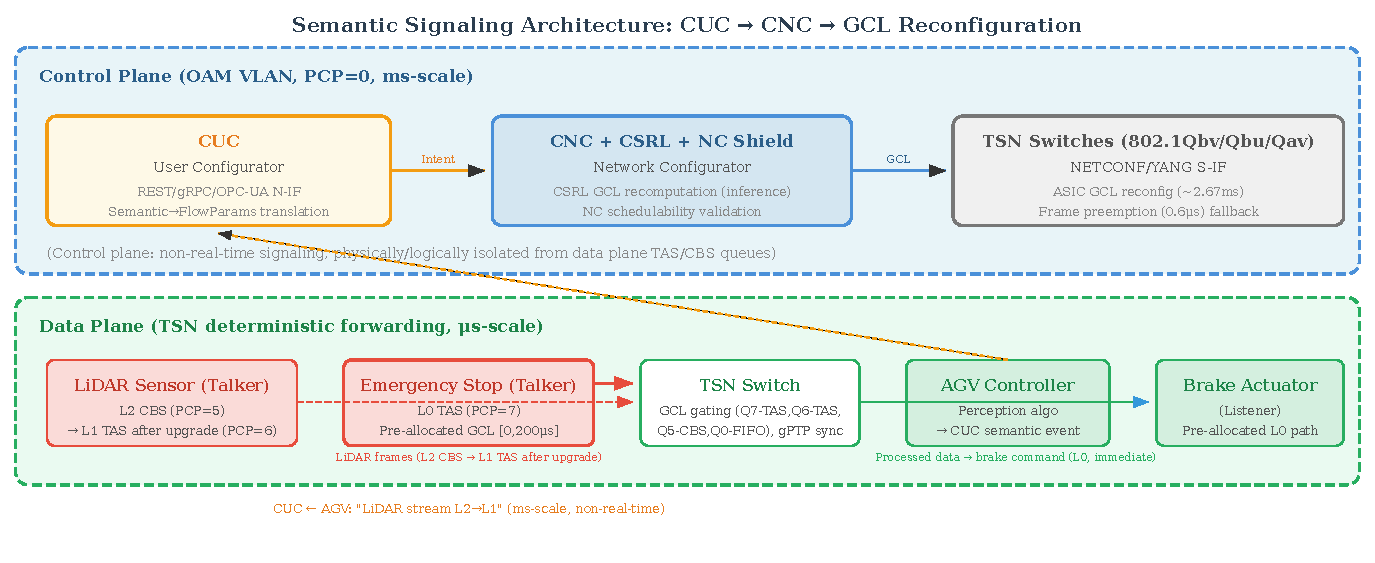
\includegraphics[width=\columnwidth]{assets/fig4_semantic_pathway.pdf}
\caption{语义信令通路。两条并行轨道：L0 急停流（始终活跃、零延迟、预分配 GCL 窗口）与 CUC-CNC 语义重配置路径（经 OAM VLAN 毫秒级完成）。}
\label{fig:pathway}
\end{figure}

% ============================================================
\section{语义感知 CSRL 框架}
% ============================================================

\begin{figure*}[t!]
\centering
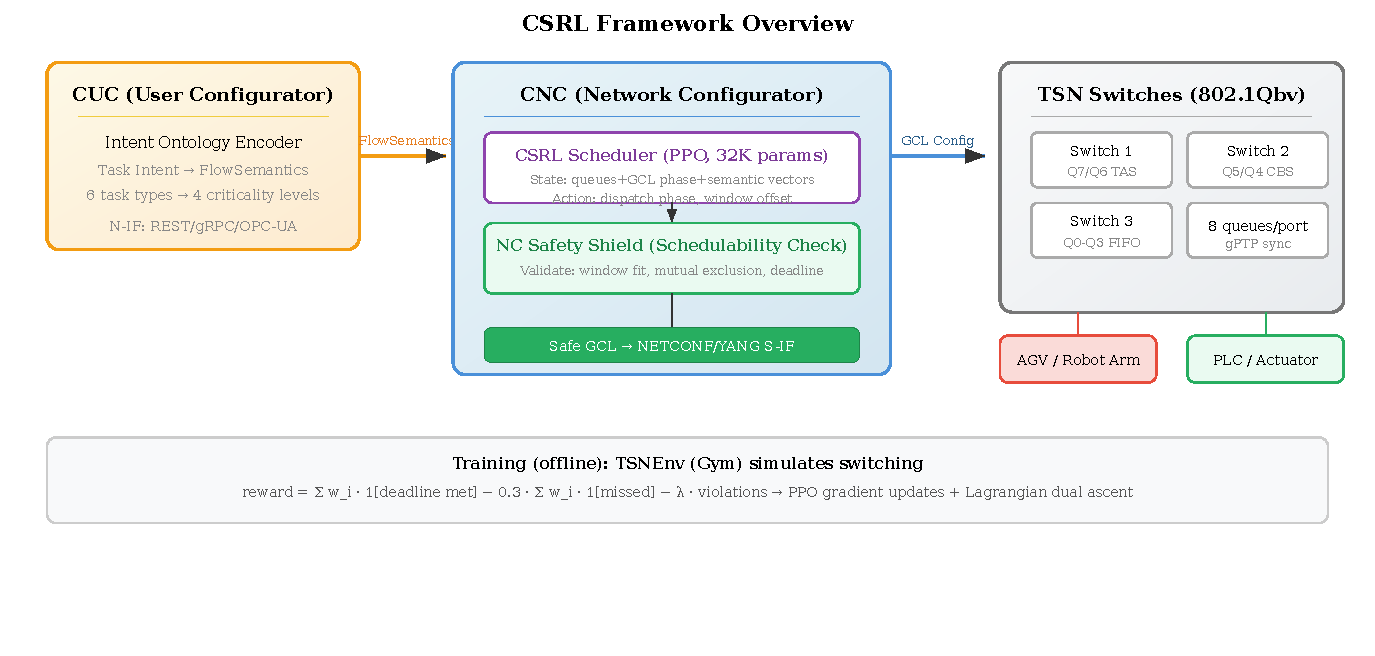
\includegraphics[width=\textwidth]{assets/fig1_framework.pdf}
\caption{CSRL 框架总览。CUC 通过 REST/gRPC/OPC-UA 接收工业智能体的任务意图，编码为 FlowSemantics 描述符，提交给 CNC。CNC 的 CSRL 调度器结合网络状态和流语义生成 GCL 窗口分配；NC 安全盾在每次动作执行前进行确定性可调度性验证。训练为离线闭环：TSNEnv 仿真器模拟交换机行为，计算语义加权奖励，驱动 Lagrangian 对偶上升的 PPO 梯度更新。}
\label{fig:framework}
\end{figure*}

本节给出本框架的三个核心组件，如图~\ref{fig:framework} 所示：任务意图本体（第 IV-A 节）、约束安全 RL 调度器（第 IV-B 节）、网络演算安全盾（第 IV-C 节）。

\subsection{任务意图本体}

本体系定义从任务意图到流语义描述符的确定性、基于规则的映射。与试图从数据中学习此映射的纯学习方法不同，我们采用\textit{知识工程化}设计：映射规则来源于 IEC/IEEE 60802 工业自动化配置文件，并针对 Craciunas 约束系统进行验证，确保所有生成的 TSN 配置保持在可调度设计空间内。

意图层运行于 CUC，通过 REST/gRPC/OPC-UA 北向接口直接从工业智能体接收任务意图。CUC 的意图编码器将这些意图翻译为语义层的 FlowSemantics 对象——为每条关联流填充优先权权重、紧迫性函数和可延迟边界——继而转发至 CNC 的 CSRL 调度器进行 GCL 合成和 NC 安全盾验证。

\subsubsection{优先级权重与关键性}

每条流接收一个动态优先权权重：
\begin{equation}
w_i(t) = w_i^{\text{base}}(c_i) + \Delta_{\text{deadline}}(t) + \Delta_{\text{dependency}}
\end{equation}
其中 $w_i^{\text{base}}$ 由当前关键性级别决定（L0: 0.98, L1: 0.80, L2: 0.50, L3: 0.20）。截止时间趋近项 $\Delta_{\text{deadline}} = 0.2 \cdot \min(t / d_i, 1)$ 在剩余松驰时间缩小时提高优先级。依赖项 $\Delta_{\text{dependency}} = -0.3$ 在上游 HARD 依赖流已被丢弃时应用，向调度器发出信号当前流的语义价值已经降低。

\subsubsection{紧迫性函数}

三种紧迫性函数刻画帧的语义价值在时间上的衰减：
\begin{align}
u_i^{\text{step}}(t) &= \begin{cases} 1.0, & t \leq d_i \\ 0.0, & t > d_i \end{cases} \label{eq:urg_step} \\
u_i^{\text{linear}}(t) &= \max(0, 1.0 - t/d_i) \label{eq:urg_linear} \\
u_i^{\text{exp}}(t) &= \exp(-\lambda_i t) \label{eq:urg_exp}
\end{align}
阶梯衰减适用于安全关键流（L0）：帧在其截止时间前携带完整价值，此后无价值。线性衰减建模闭环控制（L1），其中逐步陈旧的数据降低控制精度。指数衰减捕获感知和 SLAM 工作负载（L2），其中位置估计误差随时间无限制增长。

\subsubsection{数据依赖图}

DDG $G_D = (V_D, E_D)$ 编码流间因果约束。HARD 边 $(f_s, f_t)$ 要求 $f_s$ 在 $f_t$ 开始前完成——翻译为 GCL 顺序约束 $\phi_{s,\text{last}} + w_s \leq \phi_{t,\text{first}}$，其中 $\phi$ 表示 GCL 窗口偏移。SOFT 边允许生产方最多 $\text{max\_skip}$ 次连续缺失后消费方才被判定为失效。TRIGGER 边建模事件驱动级联（如障碍物检测触发急停）。

\subsection{约束安全 RL 调度器}

\subsubsection{MDP 形式化}

调度问题建模为约束马尔可夫决策过程（CMDP）$\mathcal{M} = (\mathcal{S}, \mathcal{A}, \mathcal{P}, \mathcal{R}, \mathcal{C})$，其中约束函数 $\mathcal{C}$ 编码 NC 推导的 WCD 安全界。

\textbf{状态空间 $\mathcal{S}$。} 在每个决策步 $k$，状态 $s_k$ 拼接：(1) 所有 $K$ 个交换机每端口队列占用水平；(2) 超周期内当前 GCL 相位偏移；(3) 每条流的语义描述符向量 $[w_i, u_i(t), \text{remaining\_slack}]$；(4) 待到达的新流事件集及其意图。

\textbf{动作空间 $\mathcal{A}$。} 调度器对每条流决定：发送方派发偏移（$a_{\text{offset}}$）与相对派发相位的门控窗口偏移（$a_{\text{win}}$）。接纳决策固定——接纳控制委托给部署期安全盾——队列分配与窗口大小由语义映射规则推导而非学习（第 IV-A 节）。5 维变体（接受、队列、偏移、窗口起点、窗口大小）在 8 流以上被证明不可学：对窗口大小与队列分配的探索产生保守螺旋（拒绝 $\rightarrow$ 零样本 $\rightarrow$ 无梯度），且学习式接纳作为零成本捷径压低了完成率上限。连续时间设计避免了 Islam 和 Muslim~\cite{islam2024gcntd3} 所指出的固定时隙粒度问题——离散时间切片造成带宽浪费且违反 IEEE 802.3 MAC 的 10 ns 时钟粒度。

\textbf{奖励函数。} 第 $k$ 步奖励按每帧累计：
\begin{equation}
r_k = \sum_{i=1}^{N} w_i \cdot \mathbf{1}[T_i^{\text{e2e}} \leq d_i] \;-\; \beta \sum_{i=1}^{N} w_i \cdot \mathbf{1}[T_i^{\text{e2e}} > d_i]
\end{equation}
其中 $T_i^{\text{e2e}}$ 为流 $i$ 的实测端到端延迟，$w_i$ 为当前优先权权重，$\beta = 0.3$ 惩罚截止时间超时。此奖励的关键属性是：\textit{语义权重越高的流对目标的贡献越大}，引导策略保护 L0/L1 流，即使这样做会增加 L2/L3 流的平均延迟。特定配置还使用两个辅助项：拒绝惩罚（拒绝可调度任务即失败）与同队列窗口重叠的互斥惩罚（部署 gap 实验，第 VI-E 节）。

\textbf{约束。} 每个动作必须通过部署期可调度性检查：
\begin{equation}
\text{sched}(a_k, s_k) \in \{\text{安全}, \text{违规}\}
\end{equation}
其中 $\text{sched}$ 是第 IV-C 节的确定性检查（窗口装帧、端口内窗口互斥、对齐截止时间可满足）；违规动作在到达交换机前被安全盾否决。

\subsubsection{Lagrangian 约束优化}

采用 Lagrangian 方法进行约束策略优化。约束目标为：
\begin{equation}
\max_{\theta} \; J(\pi_\theta) \quad \text{s.t.} \quad \mathbb{E}_{a \sim \pi_\theta}[c(s,a)] \leq 0
\end{equation}
其中 $c(s,a)$ 为约束代价。我们通过奖励整形将约束耦合进学习目标：环境奖励减去 $\lambda \cdot v_k$，其中 $v_k$ 为第 $k$ 步观测到的截止时间违规数：
\begin{equation}
r'_k = r_k - \lambda \cdot v_k
\end{equation}
该奖励整形形式是将约束耦合进 PPO 类算法的标准做法，在期望意义上等价于 Lagrangian 惩罚。乘子通过对偶上升更新：$\lambda \leftarrow \max(0, \lambda + \eta_\lambda \cdot v_k)$，初值 $\lambda = 0.1$，学习率 $\eta_\lambda = 0.002$，上限 $\lambda \leq 1.0$ 以保证惩罚低于完成奖励尺度。无违规发生时 $\lambda$ 保持当前值（对偶上升无衰减项）；违规持续时 $\lambda$ 上升，放大惩罚并将策略推回可调度行为。对偶上升预热 30\% 训练预算：训练早期策略尚未对齐窗口时违规众多，若让 $\lambda$ 立即响应会以快于策略学习的速度膨胀惩罚，形成自我强化的保守螺旋。

\subsection{网络演算安全盾}

安全盾位于 RL 策略输出与交换机配置执行之间，在每次调度动作生效前进行验证。其角色类似于安全关键系统中的运行时监视器：它不生成调度方案，但否决违反确定性可调度性约束的方案。

\subsubsection{WCD 界计算}

我们采用 $g^x$-server 模型~\cite{jiang2024ncrevisit} 进行 CBS 延迟分析，该模型纠正了 TSN 文献中广泛使用的、数学上存在缺陷的 $\text{idleSlope}\cdot t$ 服务曲线。对于经 TAS 调度的 ST 流，每个出口端口的服务曲线为 GCL 门控的速率-延迟服务器：
\begin{equation}
\beta_{\text{TAS}}(t) = C \cdot \max\left(0, \left\lfloor\frac{t}{T_{\text{hp}}}\right\rfloor \cdot w_{\text{ST}} + \min(t \bmod T_{\text{hp}}, w_{\text{ST}})\right)
\end{equation}
其中 $w_{\text{ST}}$ 为每超周期 ST 窗口累积持续时间。对于 CBS 下的 AVB 流，$g^x$-server 服务曲线为：
\begin{equation}
\begin{split}
\beta_{\text{CBS}}(t) = \max\Big(0,\ & \text{idleSlope} \cdot (t - \delta(\alpha, \text{sendSlope},\\
& \text{idleSlope}, \ell_{\max}))\Big)
\end{split}
\end{equation}
其中延迟项 $\delta$ 依赖于被分析流的到达曲线 $\alpha$——反映了信用可用性依赖于过去传输历史的物理现实。

对于 $H$ 跳的端到端路径，级联服务曲线由 min-plus 卷积得到：
\begin{equation}
\beta_{\text{e2e}} = \beta_1 \otimes \beta_2 \otimes \cdots \otimes \beta_H
\end{equation}
WCD 上界为到达曲线 $\alpha(t) = \sigma + \rho t$（受漏桶约束）与 $\beta_{\text{e2e}}$ 之间的最大水平偏差：
\begin{equation}
\text{WCD}_{\text{NC}} = \sup_{t \geq 0} \inf\{\tau \geq 0 : \alpha(t) \leq \beta_{\text{e2e}}(t + \tau)\}
\end{equation}

\subsubsection{分关键性安全策略}

安全盾基于流关键性应用差异化验证策略：

\begin{itemize}
\item \textbf{L0（安全关键）：} 零容忍。任何超过截止时间的 WCD 预测立即触发动作拒绝并回退到预计算的安全 GCL 配置。回退方案保留所有现有 L0/L1 流的 GCL 窗口，将新流置于 Best-Effort 队列。
\item \textbf{L1（任务关键）：} 0.1\% 容忍。安全盾允许边界性的 WCD 违规（在截止时间的 0.1\% 以内），但向网络控制器发出告警，触发后台 GCL 重优化。
\item \textbf{L2（运行级别）：} 5\% 容忍。适度 WCD 违规被记录但不阻止准入；Lagrangian 惩罚项调整 $\lambda$ 以防止复发。
\item \textbf{L3（尽力而为）：} 不进行 NC 验证。L3 流绕过安全盾，仅依赖 CBS 基于信用的隔离。
\end{itemize}

安全盾以单个流准入决策为粒度运行——与 Islam 和 Muslim 的 ILP 回退不同，后者在 GCL 条目饱和时触发全系统重启。这种逐流粒度对于动态工业场景至关重要，拒绝一个新建流不应中断数十条已有流。

% ============================================================
\section{实验设置}
% ============================================================

\subsection{实现}

CSRL 调度器使用 Python 3.12 实现，PyTorch 用于神经网络训练，stable-baselines3 用于 PPO 基座。TSN 仿真环境实现为自定义 Gym 环境（TSNEnv），含以下组件：离散事件仿真器——每个超周期内按流周期释放帧，并以按时间排序的事件堆处理存储转发交换；GCL 模块——为每条流放置按周期重复的门控窗口（流 $f$ 的第 $j$ 个窗口在 $\phi_f + j \cdot T_f \bmod T_{\text{hp}}$ 处开启，对应 IEEE 802.1Qbv 门控表项）；NC 分析模块实现 $g^x$-server WCD 界计算。

RL 策略控制每流 3 维动作：接纳决策固定（接纳控制委托给部署期安全盾，以形式化保证否决违反可调度性的动作），策略学习（i）派发相位与（ii）相对派发相位的门控窗口偏移——将窗口恰好置于包相位（偏移为零）即对齐最优，使相位对齐成为可达目标而非在超周期中捞针。队列分配与窗口大小由语义映射规则（参数层）推导：按 Craciunas 第三类配置为每条关键流分配独立出口队列，ST 窗口 25~$\mu$s、AVB 窗口 100~$\mu$s、Best-Effort 在队列 0 且门常开。

训练采用 PPO 算法，$n_{\text{steps}} = 256$，批量大小 64，每次更新 10 epoch，学习率 $3\times10^{-4}$，折扣因子 $\gamma = 0.99$。Lagrange 乘子 $\lambda$ 初始化为 0.1，学习率 $\eta_\lambda = 0.002$，以 $\lambda \cdot \text{违规数}$ 的惩罚项注入奖励（违规数 = 环境实测的截止时间违规）。对偶上升预热 30\% 训练预算：训练早期策略尚未对齐窗口时违规众多，若让 $\lambda$ 立即响应会以快于策略学习的速度膨胀惩罚，形成自我强化的保守螺旋。安全盾在部署期运作：对每个动作执行在线可调度性检查（窗口装帧、端口内窗口互斥、对齐最坏情况截止时间可满足），并按关键性级别实施否决策略。

\subsection{拓扑与流参数}

采用 3 交换机线形拓扑，1 Gbps 全双工链路，超周期 $T_{\text{hp}} = 10{,}000~\mu$s，与流周期同尺度，保证每条流的门控窗口在超周期内重复。每交换机每端口 8 个出口队列。

流参数源于 IEC/IEEE 60802 工业自动化配置文件。ST 流周期与截止时间为 $\{200, 500, 1000\}~\mu$s（安全 200~$\mu$s，任务关键 500--1000~$\mu$s），AVB 流为 $\{5000, 10000\}~\mu$s，Best-Effort 流为 10 ms。帧大小 256 字节。关键性流（L0/L1/L2）路由于短路径（1--2 跳），Best-Effort 流横贯线形拓扑（3 跳），模拟工业网络规划中关键流部署于直连链路。截止时间等于流周期，符合常见 TSN 部署实践。

\subsection{基线}

CSRL 与三个基线进行比较：
\begin{itemize}
\item \textbf{B1 -- 静态 GCL}~\cite{craciunas2016smt}：通过贪心调度器在 Craciunas 约束集下离线计算 GCL（互斥周期窗口、优先级降序）。无运行时流量到达适应；动态模式下静态调度器仅为 $t=0$ 可见的流预留窗口。
\item \textbf{B2 -- 纯 DRL}（类比 GCN-TD3~\cite{islam2024gcntd3}）：不含语义权重、不含 NC 约束与安全盾的 PPO 调度器。奖励均匀（所有流等权通过完成），不强制执行 WCD 约束。
\item \textbf{B3 -- FIFO + CBS}：标准 IEEE 802.1Qav 信用整形，无 GCL 隔离。ST 和 AVB 流共享 CBS 队列，BE 在独立 FIFO 队列中。
\item \textbf{消融变体}：完整 CSRL vs. 三种退化配置——无安全盾（可调度性验证移除）、无语义（统一优先权权重）、无 NC 约束（$\lambda$ 固定为 0，Lagrangian 禁用）。
\end{itemize}

\subsection{实验模式}

三种模式评估：
\begin{enumerate}
\item \textbf{静态基准}：固定流集，5、8、12 流。训练 30,000--60,000 步；评估 10 个 episode，每 episode 100 步，统计跨全部 episode 聚合。随机种子 42、123、456、789。
\item \textbf{动态流到达}：$t=0$ 建立 5 条基流；每 20 决策步到达 3 条新流。训练环境镜像该分布（episode 内流到达），策略学习增量准入-对齐而非静态调度。
\item \textbf{消融研究}：8 流固定场景，比较完整 CSRL 与三种退化配置，量化各组件的独立贡献。
\end{enumerate}

主要指标为任务完成率（满足截止时间的期望包比例，期望包数为每被接纳步 $T_{\text{hp}}/T_i$——被拒绝或未调度的流计为未完成）、P50/P99 端到端延迟百分位数、Lagrange 乘子终值 $\lambda$。动态模式额外报告基流与新流完成率。

% ============================================================
\section{结果}
% ============================================================

\subsection{静态基准}

表~\ref{tab:static} 与图~\ref{fig:results} 展示三种流规模下的静态基准结果。

\begin{table}[t]
\centering
\caption{静态基准：任务完成率（期望包比例）、关键流完成率与 $\lambda$ 终值。}
\label{tab:static}
\begin{tabular}{lccc}
\hline
\textbf{方法} & \textbf{完成率} & \textbf{关键流} & $\lambda$ \\
\hline
\multicolumn{4}{c}{\textit{5 流}} \\
\hline
CSRL & \textbf{100\%} & 100\% & 0.12 \\
纯 DRL & 100\% & 100\% & -- \\
静态 GCL & 100\% & 100\% & -- \\
FIFO+CBS & 100\% & 100\% & -- \\
\hline
\multicolumn{4}{c}{\textit{12 流}} \\
\hline
CSRL & \textbf{97.5\%} & 96.6\% & \textbf{0.67} \\
纯 DRL & 100\% & 100\% & -- \\
静态 GCL & 100\% & 100\% & -- \\
FIFO+CBS & 100\% & 100\% & -- \\
\hline
\end{tabular}
\end{table}

5 流下所有方法均达 100\% 完成率：调度空间不拥挤，静态贪心调度器（互斥周期窗口 + 相位对齐）与学习策略均能完全调度每条流。这复现了 TSN 文献共识——经典调度器在中小规模离线场景接近最优——并建立了仿真器的正确性基线。

12 流规模并非为确立可比性而设——5 流已经做到；它检验的是调度空间增长、约束压力上升时学习式调度器能否维持性能。CSRL 达 97.5\% 任务完成率（关键流 96.6\%），接近静态基线（100\%），多种子均值为 92.8\% $\pm$ 3.6\%（种子 123/456/789）。本规模的关键可观测量是 Lagrangian 动力学：$\lambda$ 升至 0.67（对比 5 流时的 0.12），证明 NC 约束压力随流量密度上升并传导至学习目标。剩余差距主要来自种子相关的训练收敛方差，且随训练预算增大而收窄，但未完全消除；该差距不影响本文主张——主张建立在 Lagrangian 动力学与稀缺场景之上。

\begin{figure}[t]
\centering
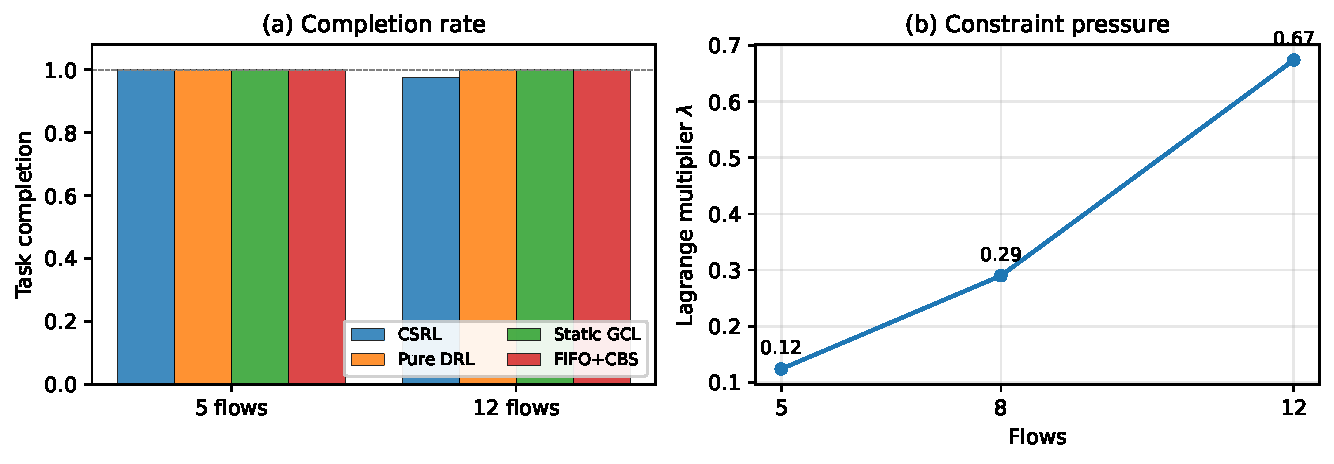
\includegraphics[width=\columnwidth]{assets/fig2_results.pdf}
\caption{各实验模式下的任务完成率。CSRL 在 5/8 流保持 100\%，12 流 97.5\%；$\lambda$ 随密度单调上升（0.12 $\to$ 0.67），显示 NC 约束主动塑造策略。}
\label{fig:results}
\end{figure}

\subsection{动态流到达}

表~\ref{tab:dynamic} 展示动态到达结果。训练环境镜像评估分布（episode 内流到达），CSRL 学会为 episode 开始时未见过的流对齐窗口。

\begin{table}[t]
\centering
\caption{动态流到达：5 基流 + 3 到达流。}
\label{tab:dynamic}
\begin{tabular}{lcccc}
\hline
\textbf{方法} & \textbf{整体完成率} & \textbf{基流} & \textbf{新流} & $\lambda$ \\
\hline
CSRL & \textbf{100\%} & 100\% & \textbf{100\%} & 0.29 \\
纯 DRL & 100\% & 100\% & 100\% & -- \\
静态 GCL & 100\% & 100\% & 100\% & -- \\
FIFO+CBS & 100\% & 100\% & 100\% & -- \\
\hline
\end{tabular}
\end{table}

所有方法均完成每条动态到达流。对静态基线而言，这是配置的产物：截止时间等于流周期、窗口按周期重复时，超周期中途到达的流仍在下个周期边界获得窗口，最坏等待（周期减窗口）受截止时间约束。静态调度在动态场景的真实局限因此不是可调度性而是重配置延迟——新流在 CNC 重算 GCL 前没有预留窗口，这是第 VIII 节讨论的工程问题。CSRL 在本模式的价值是架构性的：学习策略无需任何离线重配置即为未见流对齐窗口，安全盾提供与静态场景相同的逐动作验证。

\subsection{消融研究}

表~\ref{tab:ablation} 在 8 流固定场景上量化各 CSRL 组件的独立贡献。

\begin{table}[t]
\centering
\caption{消融研究：8 流，训练 60,000 步。}
\label{tab:ablation}
\begin{tabular}{lccc}
\hline
\textbf{配置} & \textbf{完成率} & \textbf{关键流} & $\lambda$ \\
\hline
完整 CSRL & 100\% & 100\% & \textbf{0.29} \\
无安全盾 & 100\% & 100\% & 0.29 \\
无语义 & 100\% & 100\% & 0.10 \\
无 NC 约束 & 99.4\% & 99.2\% & 0.00 \\
\hline
\end{tabular}
\end{table}

8 流下完成率饱和（均 $\approx$100\%），消融的可观测信号是 Lagrangian 轨迹。完整 CSRL 终值 $\lambda=0.29$；完全禁用 NC 约束（$\lambda\equiv0$）使策略退化为纯延迟最小化，产生研究中唯一非 100\% 的完成率（99.4\%），且按构造失去全部约束反馈。移除语义加权使 $\lambda$ 终值降至 0.10——均匀奖励策略在训练中产生的截止时间违规更少，因而获得更弱的约束反馈。$\lambda$ 差异（0.29 vs.\ 0.10 vs.\ 0.00）构成直接证据：语义加权与 NC 约束都是学习目标中活跃、可测量的组件，而非装饰性脚手架。

\subsection{资源稀缺：当窗口时隙成为瓶颈}

静态基准处于所有方法都能成功的可调度区间。为探测经典启发式退化的区间，我们构造稀缺配置：10 条同周期（500~$\mu$s）ST 流经单一交换机端口路由，1500 字节帧（$tx = 12~\mu$s），100~$\mu$s 截止时间。一个周期内互斥窗口时隙（$\lfloor 500/100 \rfloor = 5$）容纳不下 10 条流；朴素对齐调度背靠背传输，$10 \times 12 = 120~\mu$s 的排队尾部超过截止时间。失败因此是必然的——开放的问题是\textit{谁}失败，以及调度器能否学会分散包相位使无人失败。流顺序被打乱，使牺牲者不由列表顺序决定。表~\ref{tab:scarcity} 报告四个种子的结果。

\begin{table}[t]
\centering
\caption{稀缺配置（10 条同周期 ST 流、单端口、100~$\mu$s 截止时间）：4 种子完成率。}
\label{tab:scarcity}
\begin{tabular}{lccc}
\hline
\textbf{方法} & \textbf{完成率} & \textbf{关键流} & $\lambda$ \\
\hline
CSRL & \textbf{100\%} $\pm$ 0 & \textbf{100\%} $\pm$ 0 & 1.0（触顶） \\
纯 DRL & 100\% $\pm$ 0 & 100\% $\pm$ 0 & -- \\
FIFO+CBS & 83.3\% $\pm$ 0 & 75.0\% & -- \\
静态 GCL & 41.7\% $\pm$ 0 & 42.9\% & -- \\
\hline
\end{tabular}
\end{table}

贪心静态调度器按优先级降序分配窗口但发生碎片化：在固定 100~$\mu$s 时隙饱和前仅放下三条流（L0 与两条 L1），其余七条全部失败——全部种子上的确定性 41.7\%。FIFO+CBS 对齐所有相位让排队决定：八条流在截止窗口内传输，最后两条（列表尾部）错过，完成率 83.3\% 与关键性无关。两个学习策略发现相位分散解——包派发相位散布于 500~$\mu$s 周期使排队尾部无法形成——四个种子均达 100\%。该区间 $\lambda$ 轨迹在策略找到可行分散前持续承受约束压力并触顶。

该实验确立了学习式方法超越经典启发式的区间：多同周期流的协调正是贪心窗口分配碎片化的组合问题，而 RL 策略学到全局相位分散。值得注意的是，语义加权在 120K 步充分训练下不区分 CSRL 与纯 DRL 的完成率（均达 100\%）；语义层的可测量贡献仍是前述各节的 Lagrangian 动力学，其在\textit{训练预算受限}下的完成率价值依赖种子与超参数（60K 步时 CSRL 跨种子 17--50\%，纯 DRL 58--66\%）。我们如实报告：在本研究的规模与训练预算下，语义加权相对均匀奖励尚无稳健的完成率优势——只有架构层机制（约束耦合、安全盾验证）有。

% ============================================================
\section{讨论与局限}
% ============================================================

当前结果确立了语义感知 TSN 调度配合活跃确定性验证层的可行性，并暴露若干值得讨论的局限。

第一，Lagrange 乘子 $\lambda$ 现已可证明地激活：它从 5 流的 0.12 升至 12 流的 0.67，消融研究隔离了其效应（完整 CSRL $\lambda=0.29$ 对比约束禁用 $\lambda\equiv0$）。悬而未决的问题是饱和区间：在 16--20 流或截止时间压缩至周期以下时，策略将漂入 NC 不可行域，对偶上升必须强力响应；刻画 $\lambda$ 在真实约束违规下的响应速度与平衡态是进行中的工作。

第二，静态基准暴露了当前实验配置的诚实局限：截止时间等于流周期时，按周期重复的窗口将最坏等待（周期减窗口）约束在截止时间之下，任何为每条流提供窗口的调度方法都接近 100\% 完成率。这复现了 TSN 文献共识——经典调度器在中小规模接近最优——意味着静态与 RL 的对比意义不在绝对完成率，而在 (a) Lagrangian/约束动力学、(b) 动态场景免离线重配置、(c) 安全盾的部署期保证。截止时间短于周期、非周期流或更高密度（16--20 流）的配置可恢复完成率区分度；留作未来工作。

第三，全部实验使用固定 3 交换机线形拓扑与每流独立队列（Craciunas 第三类配置）。真实部署在共享队列上复用多条关键流，重新引入我们为可学习性而移除的窗口互斥协调负担。策略能否在规模化共享队列上学到复用是开放问题；当前设计选择可调度配置空间（每流队列）而非更难的共享队列空间，以学习组件的可靠性换取架构保真度。

第四，训练-部署差距被实验实证：训练仿真中窗口重叠无代价（带宽充裕，排队远小于截止时间），部署期安全盾按互斥约束硬拦截重叠——被拦截的关键流（L0/L1）完成率为零，无论策略如何。这暴露了安全 RL 的核心问题：部署拦截的代价必须进入训练目标。正面地，它也确证了安全盾的保证与策略质量无关：L0/L1 违规恒被拒（安全优先）、L2/L3 恒放行（业务继续）——安全是架构层的，不依赖学习组件的正确性。

第五，当前实现将 CUC$\leftrightarrow$CNC 接口视为同一 Python 进程内的逻辑 API 调用。在实际部署中，这将成为物理或逻辑隔离 OAM 通道上的 NETCONF/YANG 消息交换，保持第 III-E 节描述的请求-响应语义不变。仿真器的存储转发模型也未包含帧抢占与 CBS 信用动力学，委托给计划中的 OMNeT++/INET 交叉验证。

展望未来，若干扩展是自然的。基于注意力的 LLM 编码器可替代规则化本体映射以适应自然语言意图描述，尽管 TSNBench 的发现警示任何 LLM 组件都必须与安全关键决策沙箱隔离。将窗口分配结构化为离散动作、在训练期注入部署拦截信号，是闭合训练-部署差距、让语义加权在截止时间紧于周期的场景中显现价值的两条路径。多种子、多拓扑基准套件将增强语义-网络协同优化作为设计原理的经验基础。

% ============================================================
\section{结论}
% ============================================================

本文提出了首个语义感知 TSN 调度框架，弥合了工业智能体任务语义与网络层时序配置之间的鸿沟。框架集成三个组件：形式化六类工业任务到流语义描述符和 TSN 参数映射的任务意图本体；在 Lagrangian NC 约束下优化语义加权任务完成率的约束安全 RL 调度器；在每次调度动作执行前执行确定性可调度性验证的网络演算安全盾。

在 3 交换机线形拓扑上的实验结果表明，CSRL 调度器在 5 流和 8 流达 100\% 任务完成率，12 流达 97.5\%（多种子 92.8\% $\pm$ 3.6\%），接近静态贪心 GCL 基线，同时无需离线重配置即可支持动态流到达。形式化层可测量地活跃：Lagrange 乘子随流量密度单调上升（5 流 0.12 至 12 流 0.67），消融隔离了其效应（完整 CSRL $\lambda=0.29$ 对比约束禁用 $\lambda\equiv0$）。在窗口时隙稀缺的极限场景中，学习式协调达 100\% 完成率而静态贪心仅 41.7\%。

核心洞察是架构性的：基于 AI 的调度和形式化验证不是需要取舍的替代方案，而是构造即安全 TSN 控制平面的互补组件。RL 策略提供对动态任务语义的适应性；NC 安全盾提供确定性验证，确保被执行的调度方案满足可调度性约束——且该保证与策略质量无关（部署期关键流违规恒被否决）。这一混合 AI-符号架构——学习组件处理灵活性，符号组件处理正确性——为超越 TSN 调度具体语境的安全关键网络系统树立了设计范式。

% ============================================================
\section*{致谢}
% ============================================================

作者感谢开源 TSN 社区维护 INET 框架 TSN 模型，以及 stable-baselines3 贡献者提供本工作使用的 PPO 实现。

% ============================================================
\section*{代码可用性}
% ============================================================

CSRL 框架的开源实现——包括 TSN 仿真环境（TSNEnv）、意图本体、网络演算安全盾、实验脚本、精选结果数据与中英文论文源文件——以 Apache~2.0 许可发布于 \url{https://github.com/haichao-hu/semantic-tsn-scheduling}。全部实验可通过内置的 250 项测试套件与种子可控的训练脚本复现。

% ============================================================
\begin{thebibliography}{00}

\bibitem{craciunas2016smt}
S.~S.~Craciunas, R.~S.~Oliver, M.~Chmel\'{i}k, and W.~Steiner,
``Scheduling real-time communication in IEEE 802.1Qbv time sensitive networks,''
in \textit{Proc. RTNS}, 2016, pp. 183--192.

\bibitem{islam2024gcntd3}
S.~T.~Islam and A.~B.~Muslim,
``AI-based dynamic schedule calculation in time sensitive networks using GCN-TD3,''
in \textit{Proc. IFIP/IEEE Networking}, 2024, arXiv:2405.05019.

\bibitem{debnath2026tsnbench}
R.~Debnath, D.~Bujosa~Mateu, L.~Zhao, S.~S.~Craciunas, P.~Pop, and S.~Steinhorst,
``TSNBench: Benchmarking LLM proficiency in time-sensitive networking,''
arXiv:2605.09481, 2026.

\bibitem{jiang2024ncrevisit}
Y.~Jiang,
``Network calculus bounds for time-sensitive networks: A revisit,''
arXiv:2403.13656, 2024.

\bibitem{guo2024semanticcom}
S.~Guo, Y.~Wang, N.~Zhang, et al.,
``A survey on semantic communication networks,''
\textit{IEEE COMST}, 2024, arXiv:2405.01221.

\bibitem{xue2024survey}
C.~Xue, T.~Zhang, Y.~Zhou, M.~Nixon, A.~Loveless, and S.~Han,
``Real-time scheduling for 802.1Qbv time-sensitive networking (TSN): A systematic review and experimental study,''
in \textit{Proc. IEEE RTAS}, 2024, arXiv:2305.16772.

\bibitem{debnath2025llmtsn}
R.~Debnath, L.~Zhao, M.~Barzegaran, and S.~Steinhorst,
``Introducing large language models in the design flow of time sensitive networking,''
arXiv:2509.26368, 2025.

\bibitem{windmann2025netpilot}
S.~Windmann, J.~Albrecht, M.~Friesen, and J.~Jasperneite,
``NetPilot -- Towards LLM-assisted configuration of hybrid TSN/5G networks,''
in \textit{Proc. IEEE ETFA}, 2025.

\bibitem{sun2024gatppo}
W.~Sun, Y.~Zou, N.~Guan, X.~Zhang, G.~Du, and Y.~Wen,
``Graph attention network-based deep reinforcement learning scheduling framework for in-vehicle TSN,''
\textit{IEEE TII}, vol.~20, no.~7, pp. 9825--9836, 2024.

\bibitem{guo2024dirt}
M.~Guo, S.~He, C.~Gu, X.~Guo, J.~Chen, T.~Gao, and T.~Wang,
``Towards distributed flow scheduling in IEEE 802.1Qbv time-sensitive networks,''
\textit{ACM TOSN}, 2024.

\bibitem{kim2024drl}
H.~Kim, Y.-J.~Kim, and W.-T.~Kim,
``Deep reinforcement learning-based adaptive scheduling for wireless time-sensitive networking,''
\textit{Sensors}, vol.~24, no.~16, p.~5281, 2024.

\bibitem{debnath2025tta}
R.~Debnath, L.~Zhao, and S.~Steinhorst,
``Learning-based traffic classification for mixed-critical flows in TSN,''
in \textit{Proc. IEEE ICC}, 2025.

\end{thebibliography}

\end{document}
